\documentclass[11pt,conference]{IEEEtran}

% IEEE standard packages
\usepackage{cite}
\usepackage{amsmath,amssymb,amsfonts}
\usepackage{algorithmic}
\usepackage{graphicx}
\usepackage{textcomp}
\usepackage{xcolor}

% Extra packages
\usepackage{booktabs} % For formal tables
\usepackage{xspace}
\usepackage{pete} % For Pete's annotations

% Writing helpers
\newcommand{\hc}{hierarchical consensus\xspace}
\newcommand{\Hc}{Hierarchical consensus\xspace}
\newcommand{\sub}{subquorum\xspace}
\newcommand{\Sub}{Subquorum\xspace}
\newcommand{\subs}{subquorums\xspace}
\newcommand{\Subs}{Subquorums\xspace}
\newcommand{\sys}{Alia\xspace}
\newcommand{\roo}{root quorum\xspace}
\newcommand{\roos}{root quorums\xspace}
\newcommand{\Roo}{Root quorum\xspace}
\newcommand{\Roos}{Root quorums\xspace}

\def\BibTeX{{\rm B\kern-.05em{\sc i\kern-.025em b}\kern-.08em
    T\kern-.1667em\lower.7ex\hbox{E}\kern-.125emX}}

\begin{document}

\title{Consensus Across Continents}

\author{
\IEEEauthorblockN{Benjamin Bengfort, Rebecca Bilbro, Pete Keleher}
\IEEEauthorblockA{Department of Computer Science\\
University of Maryland, College Park, MD, USA\\
\{bengfort,rbilbro,keleher\}@cs.umd.edu}}

\maketitle

\begin{abstract}
    Eventually consistent systems can be made more consistent by reducing the time
until a write is fully replicated, improving global visibility of updates.
While gossip-based anti-entropy methods scale well, random selection of
anti-entropy partners is less than efficient.
Moreover, while eventual consistency may be consistent enough in a single data
center, geographic replication increases visibility latency and leads to
externally observable inconsistencies.
In this paper, we explore an improvement to pairwise, bilateral anti-entropy;
instead of uniform random selection, we introduce reinforcement learning
mechanisms to assign selection probabilities to replicas most likely to have
information.
The result is more efficient replication, faster visibility, and stronger
eventual consistency while maintaining high availability and partition
tolerance.

\end{abstract}

\begin{IEEEkeywords}
hierarchical consensus, geographic replication, delegated voting, strong consistency
\end{IEEEkeywords}

\section{Introduction}
% The intro seems like a very good narrative and captures all of the moving pieces
% I'm worried that we do not do enough to describe our system in a meaningful way
% Other papers like Akkio have 2 page intros though ...

It is easier than ever before to deploy geographically distributed data systems
that span continents and oceans.
These types of systems leverage data centers newly available around the globe,
increasing local performance by minimizing network distance between users and
replicas, and offering data recovery in the face of catastrophes such as floods or
earthquakes.
Specialized, high-availability data systems~\cite{megastore,tao,akkio,dynamic_placement}
have maximized throughput across the wide area, driving interest in
geo-replicated systems and making truly international applications increasingly
feasible.
To generalize geographically distributed systems, managed replicated data
services~\cite{spanner,aurora,cockroachdb} that can provide strong consistency semantics
have risen to prominence.
However, the solutions introduced by these new systems and services require specialized
hardware and engineering involving multiple independent subsystems with different
failure modes, which, while providing strong consistency to application developers, do
so by hiding both replication and infrastructure complexity.

Alia is the first distributed system of its kind to implement hierarchical consensus,
a flexible protocol that facilitates adaptation in geo-replicated distributed systems.
Hierarchical consensus comprises four key contributions; first, \emph{reconfigurable
consensus}, which allows systems to adapt to changing quorum membership, including
dynamic replacement and expansion; second, \emph{delegated voting}, which allows
decisions to be coordinated at the root (i.e. master) quorum, but executed by informed
hyperlocal subquora; third \emph{fuzzy transitions}, which allow the system to progress
unimpeded by leadership changes and reconfigurations; and finally, \emph{flexible data
placement}, which facilitates a greater proportion of direct accesses.
Together, these four features offer strong consistency at scale amidst dynamically
growing and shifting globally distributed systems of the kind required by modern
applications.

The engineering-based solutions of managed geo-distributed data services are designed to
coordinate hundreds of replicas that have access to expensive data-center hardware and
involves multiple, independent processes and quorums to synchronize time, allocate locks,
manage transactions, and recover from failure.
Meanwhile, traditional monolithic applications are being replaced by microservice
architectures and cloud-native service meshes~\cite{envoy} that make
infrastructure directly visible to applications.
As applications scale, service meshes make it easier to maintain and optimize
service-specific communication to minimize downtime and to improve system flexibility.
Additionally, due to increasing privacy regulation, application developers require more
control over data placement rather than less~\cite{gdpr}.
Thus, while managed data services provide strong consistency, they do so in an rigid, 
opaque manner that is not flexible enough for developers who require strong consistency
at a higher level of the application stack

We propose a simpler approach to building large, geographically replicated systems.
Rather than relying on a fleet of loosely-coupled, independent small quorums whose
interactions are difficult to reason about, we propose a single, system-wide consensus
protocol that coordinates both replica placement and data accesses.
By ensuring that all coordination occurs through a single consensus activity,
it is easier to reason about the consistency of the system even in a network environment
prone to correlated failures, partitions, and variable latency.
Additionally, a single source of coordination gives the system the freedom to adapt to
changes in access patterns, configure to maximize throughput, specify data placement
rules, and ensure straightforward system maintenance.

In order to achieve this, a new consensus protocol that can scale beyond a handful of
replicas is required.
Distributed consensus, canonically represented by Paxos~\cite{paxos_simple} and its
performance optimizing
variants~\cite{fast_paxos,multicoordinated_paxos,spaxos,generalized_paxos}, primarily
consider safety in the case of one or two fail-stop node failures.
Although some recent research has explored the problem of geo-distributed
consensus~\cite{mencius,epaxos}, it primarily considers the problem of high-latency
links but geo-replication implies scale.
Services running around the globe require dozens if not hundreds of replicas and
introduce new failure modes such as network partitions, where sections of the system
operate independently without fail-stop failure, and highly variable latency that
inhibit quorum progress.
In order to scale systems beyond a handful of replicas, current
systems~\cite{spanner,scatter,mdcc,calvinfs} use Paxos as a component, instantiated
across multiple transactions, shards, or tablets to manage small subsystems
independently, leading to increased complexity and reduced transparency.

% the below paragraph needs help
We introduce a novel approach to scale consensus beyond a handful of nodes:
\emph{\hc}.
Our approach is to similarly decompose the consensus problem into units that can be
handled by provenly safe algorithms, but organizes all managed processes into an
intersecting hierarchy of quorums that ensure that all system-wide consensus decisions
are totally ordered.
The challenge is in building a multi-group coordination protocol that configures and
mediates \subs through a \roo.
The \roo guarantees correctness by pivoting the system through \emph{reconfigurations}
that place replicas into \subs and maps them to partitions of the object namespace to
handle direct data accesses.
The \roo is composed of all replicas in the system, although reconfigurations are rare
with respect to data accesses, we introduce \emph{delegated voting} to optimize quorum
decisions at the root.
Much of the systems complexity comes from handshaking between the \roo and \subs during
reconfiguration.
These handshakes are made easier and far more efficient by using \emph{fuzzy transitions},
which allow individual \subs to move through reconfiguration at their own pace without
impeding progress.
Finally, subquorum consensus can be optimized for policy-driven \emph{data placement},
allowing objects that require more throughput to use leader-oriented consensus whereas
objects that require stronger durability can be replicated across data centers using
optimistic fast-path consensus.

We validate our approach by implementing \hc in Alia, a linearizable object store
explicitly intended to run with many replicas, geo-replicated across heterogenous
networks and devices.
The resulting system is local, in that replicas serving clients can be located near them.
The system is fast because individual operations are served by a small group of replicas
regardless of the size of the total system.
The system is nimble in that it it can dynamically reconfigure the number, membership,
and responsibilities of the subquorums in response to failures, phase changes in the
driving applications or policy requirements for data placement and durability.
Finally, the system is consistent, supporting the strongest form of per-object
consistency without relying on special-purpose hardware.
We demonstrate its advantages through an implementation scaling to hundreds of replicas
across more than a dozen availability zones around the world using Amazon EC2.

% TODO: do we need rest of paper outline or contributions here?

% Contributions:
% - Reconfigurable consensus + adaptability
% - Delegated voting to scale consensus
% - Fuzzy transitions to allow progress
% - Access/policy optimized data placement rules

\section{Hierarchical Consensus}

\begin{figure}[t]
    \centering
    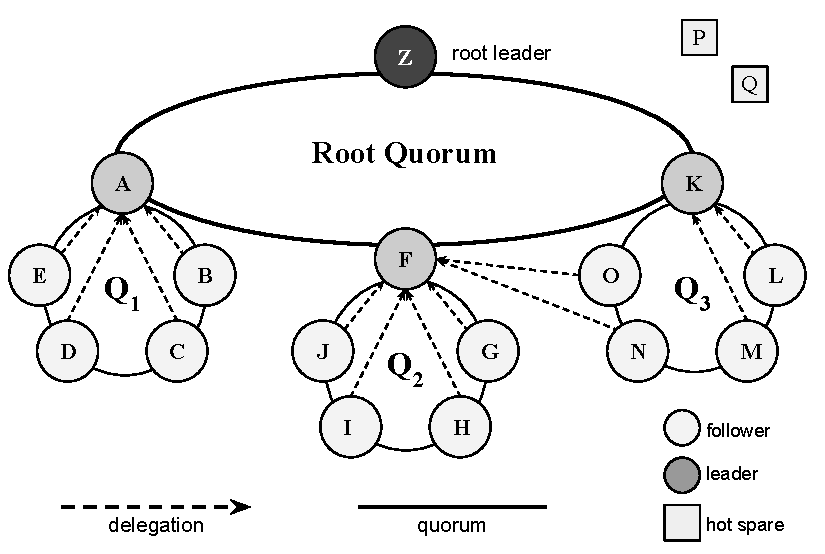
\includegraphics[width=0.48\textwidth]{figures/election3}
    \caption{Replicas participate in intersecting tiers of consensus.}
    \label{fig:system}
\end{figure}

Hierarchical consensus is an implementation and extension of Vertical
Paxos~\cite{vertical_paxos} that organizes replicas into two tiers of
quorums, each responsible for fundamentally different decisions, as shown
in Figure \ref{fig:system}.
The lower tier consists of multiple independent subquorums, each committing
operations to local shared logs.
The upper, root quorum, consists of subquorum peers, usually their leaders,
delegated to represent the subquorum and hot spares in root elections and
commits.
Hierarchical consensus's main function is to export a linearizable abstraction
of shared accesses to some underlying substrate, such as a distributed
object store or file system.
We assume that nodes hosting object stores, applications, and HC are
frequently co-located across the wide area.

The root quorum's primary responsibilities are mapping replicas to individual
subquorums and mapping subquorums to tags within the namespace.
Each such map defines a distinct epoch, $e_x$, a monotonically increasing
representation of the term of the configuration of subquorums and tags,
$Q_x$.
The root quorum is a consensus group consisting of subquorum leaders.
Somewhat like subquorums, the membership of the root quorum is not defined
by the quorum itself, but in this case by leader election or peer delegations
in the lower tier.
While the root quorum is composed of all replicas in the system, only this
subset of replicas actively participates in root quorum decision making,
in the common case.

The root quorum partitions (shards) the namespace across multiple
subquorums, each with a disjoint portion as its scope.
The namespace is decomposed into a set of tags, $T$ where each tag $t_i$
is a disjoint subset of the namespace.
% Ben: above Pete says T=t_i summation

Tags are mapped to subquorums in each epoch, $Q_x \mapsto T_x$ such that
$\forall t \in T_x$ $\exists! q_{i,x} \mapsto t$.
The intent of subquorum localization is ensure that the \emph{domain} of
a client, the portion of the namespace it accesses, is entirely within
the scope of a local, or nearby, subquorum.
To the extent that this is true across the entire system, each client
interacts with only one subquorum, and subquorums do not interact at all
during execution of a single epoch.
This \emph{siloing} of client accesses simplifies implementation of
strong consistency guarantees and allows better performance at the cost
of restricting multi-object transactions.
We use agility to attempt to get this, but allow multi-object transactions.

\subsection{Delegated Voting}
% This is about root quorum operations
From a logical perspective, the root quorum's membership is the set of
all system replicas, at all times.
However, running consensus elections across large systems is inefficient
in the best of cases, and prohibitively slow in a geo-replicated
environment.
Root quorum decision-making is kept tractable by having replicas
\emph{delegate} their votes, usually to their local leaders, for a finite
duration of epochs.
With leader delegation, the root membership effectively consists of the
set of subquorum leaders.
Each leader votes with a count describing its own and peer votes from its
subquorum and from hot spares that have delegated to it.
A quorum leader is elected to indefinitely assign log entries to slots
(access operations for subquorums, epoch configurations for the root
quorum).
If the leader fails, then so long as the quorum has enough online peers,
they can elect a new leader.
When a failed leader comes back online, it rejoins the quorum as a
follower.
The larger the size of the quorum, the more failures it is able to
tolerate.

Delegation ensures that root quorum membership is always the entire
system and remains unchanged over subquorum leader elections and even
reconfiguration.
Delegation is essentially a way to optimistically shortcut contacting
every replica for each decision.
Subquorum repartitioning merely implies that a given replica's vote
might need to be delegated to a different leader.
To ensure that delegation happens correctly and without requiring
coordination, we simply allow a replica to directly designate another
replica as its delegate until some future epoch is reached.
Replicas may only delegate their vote once per epoch and replicas are
not required to delegate their vote.
To simplify this process, during configuration of subquorums by the
root quorum, the root leader provides delegate hints, e.g. those
replicas that have been stable members of the root quorum without
partitions.
When replicas receive their configuration they can use these hints
to delegate their vote to the closest nearby delegate if not already
delegated for the epoch.
If no hints are provided, then replica followers generally delegate
their vote to the term 1 leader and hot spares to the closest subquorum
leader.

Delegation does add one complication: the root quorum leader must
know all vote delegations to request votes when committing epoch
changes.
We deal with this issue by simplifying our protocol.
Instead of sending vote requests just to subquorum leaders,
\textbf{the root quorum leader sends vote requests to all system
replicas.}
This is true even for \emph{hot spares}, which are not currently
in any subquorum.
Delegates reply with the unique ids of the replicas they represent
so that root consensus decisions are still made using a majority of
all system replicas.

This is correct because vote requests now reach all replicas, and
because replicas whose votes have been delegated merely ignore the
request.
We argue that it is also efficient, as a commit's efficiency depends
only on receipt of a majority of the votes.
Large consensus groups are generally slow, not just because of
communication latency, but because large groups in a heterogeneous
setting are more likely to include replicas on very slow hosts or
networks.
In the usual case for our protocol, the root leader still only needs
to wait for votes from the subquorum leaders.
Leaders are generally those that respond more quickly to timeouts, so
the speed of root quorum operations is unchanged.

% what happens if there is only one delegate?

\subsection{Reconfiguration}
% This is about root quorum operations

Every epoch represents a new configuration of the system as designated
by the root leader.
Efficient reconfiguration ensures that the system is both dynamic,
responding both to failures and changing usage patterns, and minimizes
coordination by colocating related objects.
An epoch change is initiated by the root leader in response to one of
several events, including:

\begin{itemize}
    \item a namespace repartition request from a subquorum leader
    \item notification of join requests by new replicas
    \item notification of failed replicas
    \item changing network conditions that suggest re-assignment of replicas
    \item manual reconfigurations, e.g. to localize data
\end{itemize}

The root leader transitions to a new epoch through the normal commit
phase in the root quorum.
The command proposed by the leader is an enumeration of the new subquorum
partition, namespace partition, and assignment of namespace portions to
specific subquorums.
The announcement may also include initial leaders for each subquorum,
with the usual rules for leader election applying otherwise, or if the
assigned leader is unresponsive.
Upon commit, the operation serves as an \emph{announcement} to subquorum
leaders.
Subquorum leaders repeat the announcement locally, disseminating full
knowledge of the new system configuration, and eventually transition to
the new epoch by committing an \texttt{epoch-change} operation locally.

The epoch change is lightweight for subquorums that are not directly
affected by the overarching reconfiguration.
If a subquorum is being changed or dissolved, however, the
\emph{epoch-change} commitment becomes a tombstone written to the logs
of all local replicas.
No further operations will be committed by that version of the subgroup,
and the local shared log is archived and then truncated.
Truncation is necessary to guarantee a consistent view of the log within
a subquorum, as peers may have been part of different subquorums, and
thus have different logs, during the last epoch.
Replicas then begin participating in their new subquorum instantiation.
In the common case where a subquorum's membership remains unchanged
across the transition, an \texttt{epoch-change} may still require
additional mechanism because of changes in namespace responsibility.

\subsection{Data Placement}

% TODO
Systems are extremely sensitive to access patterns though most applications and systems
are opnly optimized for one type of access pattern.
Real-world systems have multiple types of access patterns including:

\begin{itemize}
    \item single ownership: objects are accessed in one region and do not migrate
    \item revolving access: object accesses migrate through space and time, e.g. objects
    are more frequently accessed during daylight hours.
    \item conflicting access: objects are continuously accessed from multiple regions
\end{itemize}

Because \subs operate independently for a specific portion of the namespace for an
entire epoch, reconfiguration can be used to determine placement rules that best
optimize for access patterns and durability requirements.

To maximize throughput with no need for strong durability, a \sub can be placed in a
single region using Raft to maximize throughput.
To increase durability, data can be placed with a leader and primary backup in a single
region, and a secondary backup in a remote region.
Using this scheme it is important to modify the election rules of Raft to decrease the
probabiliy that the secondary backup is elected leader.
To handle conflicting accesses across regions, ePaxos or mencius can be used to
optimistically serialize proposals across the wide area.

\subsection{Fuzzy Transitions}

Epoch handshakes are required whenever the namespace-to-\sub mapping changes across an
epoch boundary.
HC separates epoch transition announcements in the
\roo from implementation in \subs.
Epoch transitions are termed \emph{fuzzy} because
\subs need not all transition synchronously.
There are many reasons why a \sub might be slow.
Communication delays and partitions might delay notification.
Temporary failures might block local commits.
A \sub might also delay transitioning to allow a local burst of activity to
cease such as currently running transactions\footnote{The HC protocol
discussed in this paper does not currently support transactions.}.
Safety is guaranteed by tracking \sub dependencies across the epoch boundary.

\begin{figure}[t]
    \centering
    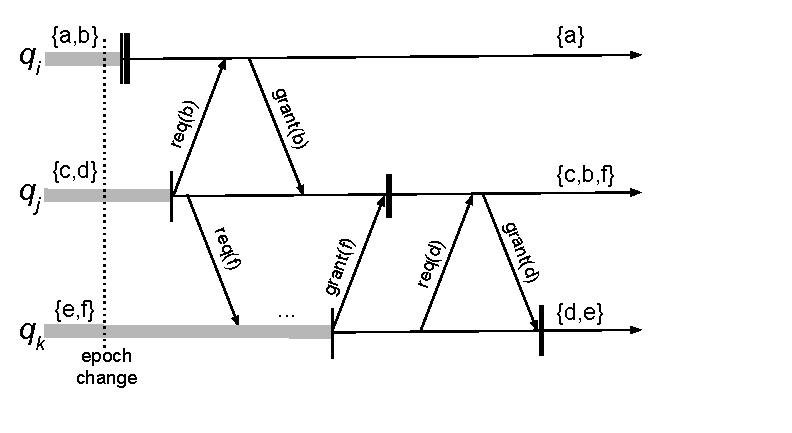
\includegraphics[width=0.48\textwidth]{figures/namespaceHandoff}
    \caption{Fuzzy transition.}
    \label{fig:handoff}
\end{figure}

Figure~\ref{fig:handoff} shows an epoch transition where the scopes of
$q_i$, $q_j$, and $q_k$ change across the transition as follows:

\begin{align*}
  \label{eq:3}
  q_{i,x-1} = t_a, t_b  &\longrightarrow q_{i,x} = t_a\\
  q_{j,x-1} = t_c, t_d  &\longrightarrow q_{j,x} = t_c,t_d,t_f\\
  q_{k,x-1} = t_e, t_f  &\longrightarrow q_{k,x} = t_d,t_e
\end{align*}

All three \subs learn of the epoch change at the same time, but become ready
with varying delays.
These delays could be because of network lags or ongoing local activity.
\Sub $q_i$ gains no new tags across the transition and moves immediately to the new epoch.
\Sub $q_j$'s readiness is slower, but then it sends requests to the
owners of both the new tags it acquires in the new epoch.
Though $q_i$ responds immediately, $q_k$ delays its response until locally
operations conclude.
Once both handshakes are received, $q_j$ moves into the new epoch, and $q_k$
later follows suit.

These bilateral handshakes allow an epoch change to be implemented
incrementally, eliminating the need for lockstep synchronization across the entire
system.
This flexibility is key to coping with partitions and varying connectivity in
the wide area.
However, this piecewise transition, in combination with \sub re-definition and
configuration at epoch changes, also means that individual replicas \emph{may
be part of multiple \subs at a time}.

This overlap is possible because replicas may be mapped to distinct subgroups
from one epoch to the next.
Consider $q_k$ in Figure~\ref{fig:handoff} again.
Assume the epochs shown are $e_x$ and $e_{x+1}$.
A single replica, $r_a$, may be remapped from \sub $q_{k,x}$ to \sub $q_{i,x+1}$ across the
transition.
\Sub $q_{k,x}$ is late to transition, but $q_{i,x+1}$ begins the new epoch
almost immediately.
Requiring $r_a$ to participate in a single \sub at a time would potentially delay
$q_{i,x+1}$'s transition and impose artificial synchronicity constraints on the
system.
One of the many changes we made in the base Raft protocol is to
allow a replica to have multiple distinct shared
logs.
Smaller changes concern the mapping of requests and responses to the appropriate
consensus group.

\section{Fault Tolerance}

We assert that consensus at the leaf replicas is correct and safe because decisions are
implemented using well-known leader-oriented consensus approaches.
Hierarchical consensus therefore has to demonstrate linearizable correctness and safety
between \subs for a single epoch and between epochs.
Briefly, linearizability requires external observers to view operations to objects as
instantaneous events.
Within an epoch, subquorum leaders serially order local accesses, thereby guaranteeing
linearizability for all replicas in that quorum.
% Remote accesses and the internal invariant also enforce linearizability of accesses
% between \subs.

Epoch transitions raise the possibility of portions of the namespace being re-assigned from one \sub to
another, with each \sub making the transition independently.
Correctness is guaranteed by an invariant requiring \subs to delay serving newly
acquired portions of the namespace until after completing all appropriate handshakes.

\begin{table*}[t]
  \centering
  \begin{tabular}{l|l} \hline
    \mcn{Failure Type} & \mcn{Response} \\ \hline
    \sub peer & request replica repartition from \roo \\
    \sub leader & local election, request replacement from \roo \\
    root leader & root election (with delegations)\\
    majority of majority of \subs & (nuclear option) root election after delegations
                                    timed out \\
  \end{tabular}
  \label{tab:categories}
\end{table*}

\subsection{Failures}

During failure-free execution, the \roo partitions the system into
disjoint \subs, assigns \emph{\sub leaders}, and assigns partitions
of the tagspace to \subs.
Each \sub coordinates and responds to accesses for objects in its assigned
tagspace.
We define the system's \emph{safety} property as guaranteeing that
non-linearizable (or non-sequentially-consistent)
event orderings can never be observed.
We define the system's \emph{progress} property as the system having enough
live replicas to commit votes or operations in the \roo.

The system can suffer several types of failures, as shown in
Table~\ref{tab:categories}.
Failures of \sub and \roo leaders are handled through the normal consensus
mechanisms.
Failures of \sub peers are handled by the local leader petitioning the \roo to
re-configure the \sub in the next epoch.
Failure of a \roo peer is the failure of \sub leader, which is handled as
above.
\Roo heartbeats help inform other replicas of leadership changes, potentially
necessary when individual \subs break down.

HC's structure means that some faults are more important than others.
Proper operation of the \roo requires the majority of replicas in the majority of \subs to
be non-faulty.
Given a system with $2m+1$ \subs, each of $2n+1$ replicas, the entire
system's progress can be halted with as few as $(m+1)(n+1)$ well-chosen
failures.
Therefore, in worst case, the system can only tolerate:
\begin{align*}
f_{worst}=mn+m+n
\end{align*}
failures and still make progress.
At maximum, HC's basic protocol can tolerate up to:
% f_{max} = (m+1)*n + m*(2n+1) = mn + n + 2mn+m = 3mn+m+n
\begin{align*}
f_{best} = (m+1)*n + m*(2n+1) = 3mn+m+n
\end{align*}
failures.
As an example, a 25/5 system can tolerate at least 8 and
up to 16 failures out of 25 total replicas.
A 21/3 system can tolerate at least 7, and a maximum of 12,
failures out of 21 total replicas.
Individual \subs might
still be able to perform local operations despite an impasse at the global level.

Total \sub failure can temporarily cause a portion of the namespace to be unserved. However, the \roo
eventually times out and moves into a new epoch with that portion assigned to another
\sub.

\subsection{The Nuclear Option}
Singleton consensus protocols, including Raft, can tolerate just under half of the entire system
failing.
As described above, HC's structure makes it more vulnerable to clustered failures.
Therefore we define a \emph{nuclear option}, which uses direct consensus
decision among all system replicas to tolerate any $f$ replicas
failing out of $2f+1$ total replicas in the system.

A nuclear vote is triggered by the failure of a root leader election.
A \emph{nuclear candidate}
increment's its term for the \roo and broadcasts a request for votes to all
system replicas.
The key difficulty is in preventing delegated votes and
nuclear votes from reaching conflicting decisions.
Such situations might occur when temporarily unavailable \sub leaders regain connectivity
and allow a wedged \roo to unblock.
Meanwhile, a nuclear vote might be concurrently underway.

Replica delegations are defined as intervals over specific slots.
Using local \sub slots would fall prey to the above problem, so we define
delegations as a small number (often one) of root slots, which usually
correspond to distinct epochs.
During failure-free operation, peers delegate to their leaders and are all
represented in the next root election or commit.
Peers then renew their delegations to their leaders by appending them to the
next local commit reply.
This approach works for replicas that change \subs over an epoch
boundary, and even allows peers to delegate their votes to arbitrary other
peers in the system (see replicas $r_N$ and $r_O$ in Figure~\ref{fig:system}).

This approach is simple and correct, but deals poorly with leader turnovers in
the \subs.
Consider a \sub where all peers have delegated votes to their leader
for the next root slot.
If that leader fails, none of the peers will be represented.
We finesse this issue by re-defining such delegations to count
root elections, root commits, \emph{and} root heartbeats.
The latter means that local peers will regain their votes for the next \roo
action if it happens after to the next heartbeat.

Consider the worst-case failure situation: a majority of the majority of \subs have
failed.
None of the failed \sub leaders can be replaced, as none of those \subs have
enough local peers.

The first response is initiated when a replica holding delegations (or its own
vote) times out waiting for the root heartbeat.
That replica increments its own root term, adopts the prior system
configuration as its own, and becomes a root candidate.
This candidacy fails, as a majority of \sub leaders, with all of their
delegated votes, are gone.
Progress is not made until delegations time out.
In our default case where a delegation is for a single root event, this
happens after the first root election failure.

At the next timeout, any replica might become a candidate because delegations have
lapsed (under our default assumptions above).
Such a \emph{nuclear} candidate increments its root term and
sends candidate requests to all system replicas,
succeeding if it gathers a majority across all live replicas.

The first candidacy assumed the prior system configuration in its candidacy
announcement.
This configuration is no longer appropriate unless some of the ``failed''
replicas quickly regain connectivity.
Before the replica announces its candidacy for a second time, however, many of
the replica replies have timed out.
The candidate alters its second proposed configuration by recasting all such
replicas as hot spares and potentially reducing the number and size of the
subgroups.
Subsequent epoch changes might re-integrate the new hot spares if the replicas
regain connectivity.

\section{Evaluation}

HC was designed to adapt both to dynamic workloads as well as variable network 
conditions.
We therefore evaluate HC in three distinct environments: a homogeneous data center, a 
heterogeneous real-world network, and a globally distributed cloud network.
The homogeneous cluster is hosted on Amazon EC2 and includes 26 ``t2.medium'' instances: 
dual-core virtual machines running in a single VPC with inter-machine latencies 
($\lambda$) normally distributed with a mean, $\lambda_{\mu}=0.399ms$ and standard 
deviation, $\lambda_{\sigma}=0.216ms$.
The heterogeneous cluster (UMD) consists of several local machines distributed across a 
wide area, with inter-machine latencies ranging from
$\lambda_{\mu}=2.527ms$,
$\lambda_{\sigma}=1.147ms$ to $\lambda_{\mu}=34.651ms$,
$\lambda_{\sigma}=37.915ms$.
The variability of this network also poses challenges that HC is uniquely suited to 
handle via root quorum-guided adaptation.
We explore two distinct scenarios -- sawtooth and repartitioning -- using this cluster; 
all other experiments were run on the EC2 cluster.

In our final experiment, we explore the use of hierarchical consensus in an extremely 
large, planetary-scale system comprised of 105 replicas in 15 data centers in 5 
continents spanning the northern hemisphere and South America. This experiment was also 
hosted on EC2 ``t2.medium`` instances in each of the regions available to us at the time 
of this writing. In this context, reporting average latencies is difficult as 
inter-region latencies depend more on network distance than can be meaningfully 
ascribed to a single central tendency.

\subsection{Basic Performance}

\begin{figure*}[t]
    \centering
    \minipage{0.5\textwidth}
        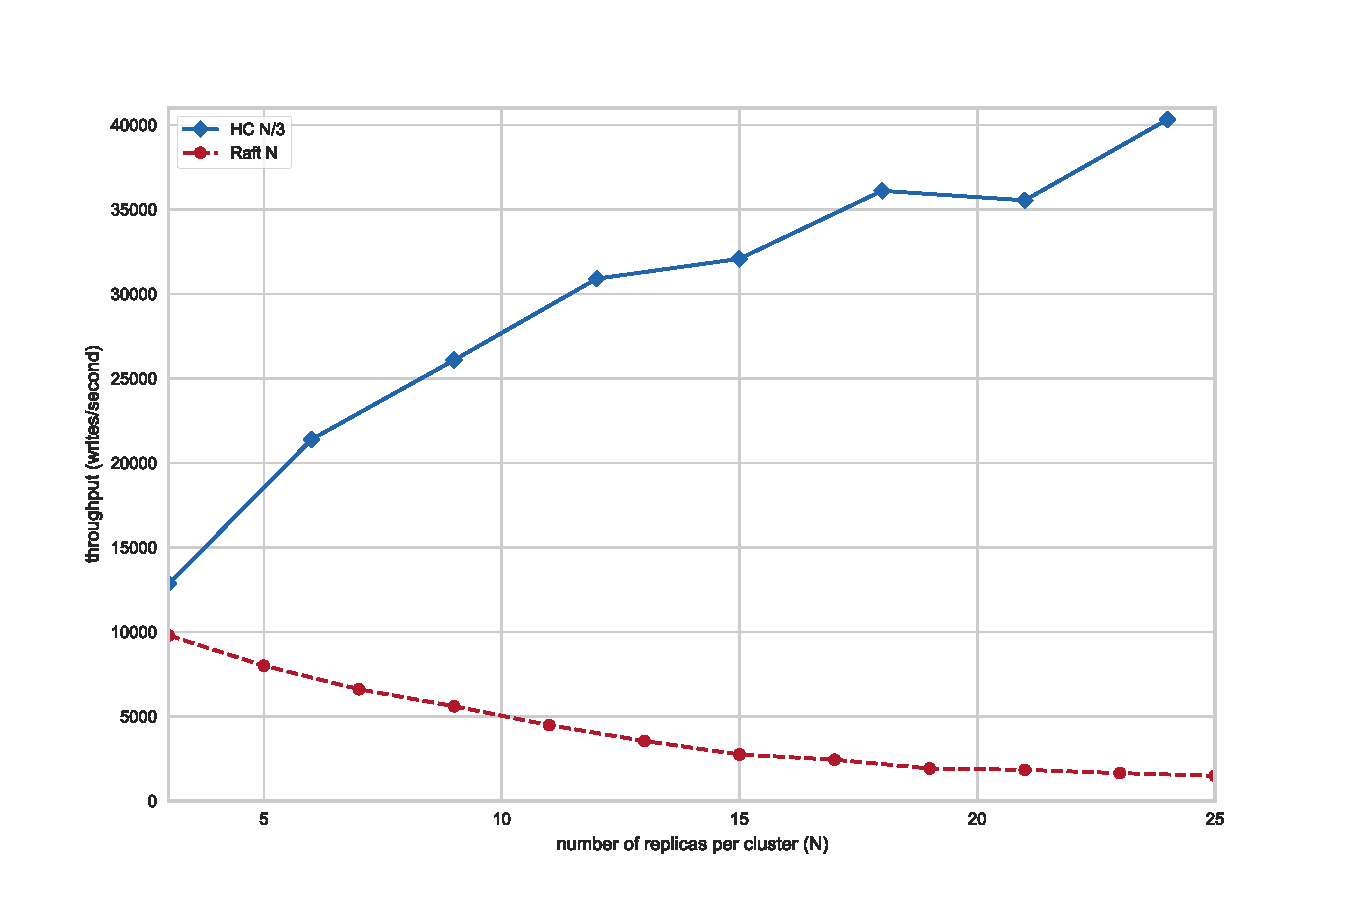
\includegraphics[width=\linewidth]{figures/scaling.pdf}
        \caption{Performance increases with larger quorum sizes}
        \label{fig:scaling_consensus}
    \endminipage\hfill
    \minipage{0.5\textwidth}%
        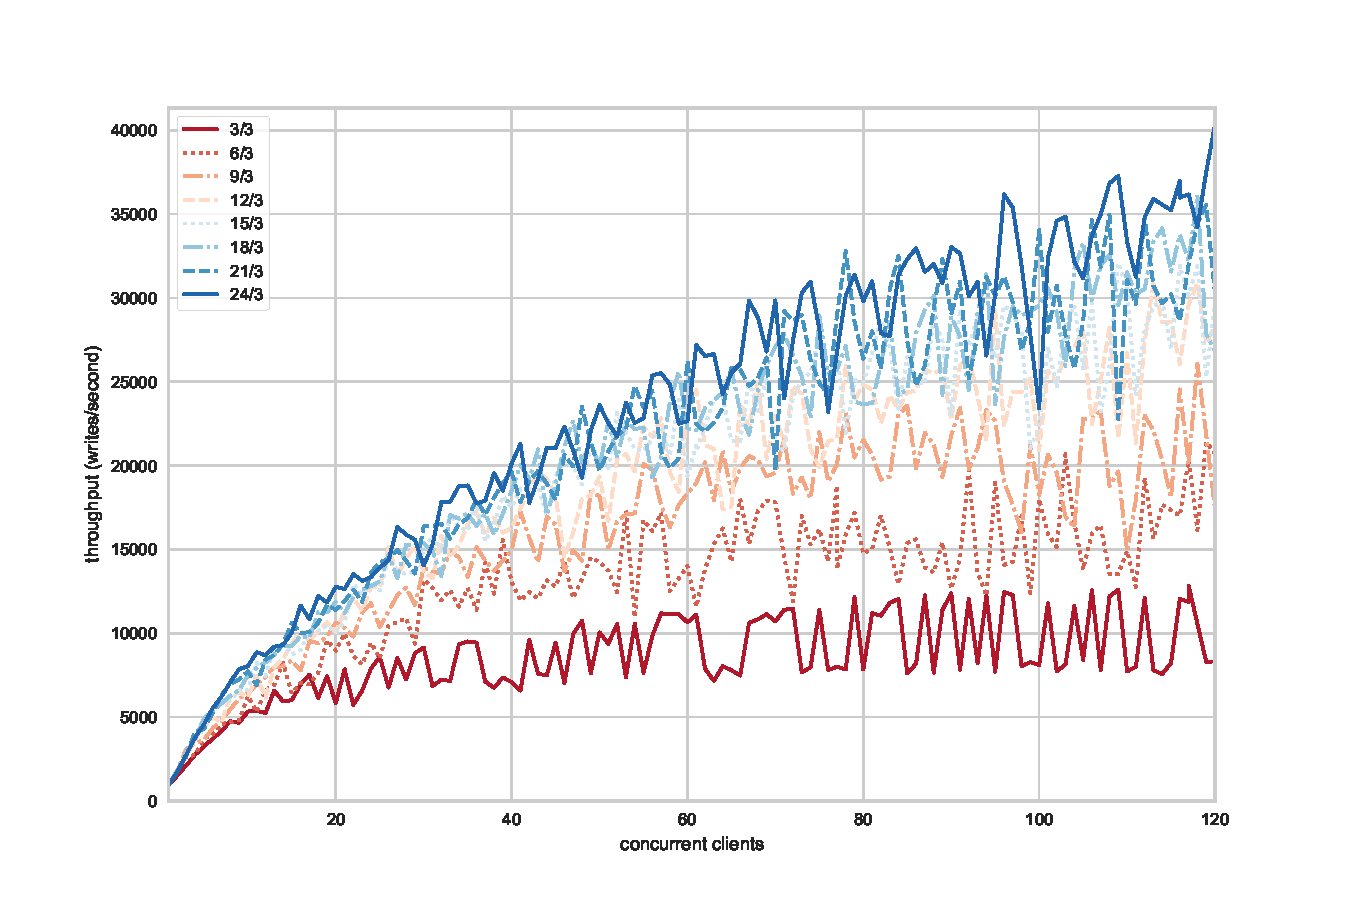
\includegraphics[width=\linewidth]{figures/hc_throughput_workload.pdf}
        \caption{Can handle larger workloads with larger system sizes}
        \label{fig:throughput_workload}
    \endminipage
\end{figure*}

HC is partially motivated by the need to scale strong consistency to large cluster sizes.
We based our work on the assumption that consensus performance decreases as the quorum 
size increases, which we confirm empirically in Figure~\ref{fig:scaling_consensus}.
This figure shows the maximum throughput against system size for a variety of workloads, 
up to 120 concurrent clients.
A workload consists of one or more clients continuously sending writes of a specific 
object or objects to the cluster without pause.

Standard consensus algorithms, Raft in particular, scale poorly with uniformly 
decreasing throughput as nodes are added to the cluster.
Commit latency increases with quorum size as the system has to wait for more responses 
from peers, thereby decreasing overall throughput.
Figures~\ref{fig:scaling_consensus} and~\ref{fig:throughput_workload} 
clearly show the multiplicative advantage of HC's hierarchical structure.
Note that though HC is not shown to scale linearly in these figures, this is due to 
performance bottlenecks of the networking implementation in these experiments.
In our final experiment, we show linear scaling with our latest implementation of HC.

There are at least two factors limiting the HC throughput shown in our initial experiments.
First, the HC subquorums for the larger system sizes are not saturated.
A single 3-node subquorum saturates at around 25 clients and this experiment has only 
about 15 clients per subquorum for the largest cluster size.
We ran experiments with 600 clients, saturating all subquorums even in the 24-node case.
This throughput peaked at slightly over 50,000 committed writes per second, better but 
still lower than the linear scaling we had expected.

We think the reason for this ceiling is hinted at by Figure~\ref{fig:throughput_workload}.
This figure shows increasingly larger variability with increasing system sizes.
A more thorough examination of the data shows widely varying performance across 
individual subquorums in the larger configurations.
After instrumenting the experiments to diagnose the problem, we determined it was a bug 
in the networking code, which we repaired and improved.
By aggregating append entries messages from clients while consensus messages were 
in-flight, we managed to dramatically increase the performance of single quorums and 
reduce the number of messages sent.
This change also had the effect of ensuring that the variability was decreased in our 
final experiment.

\begin{figure}
    \centering
    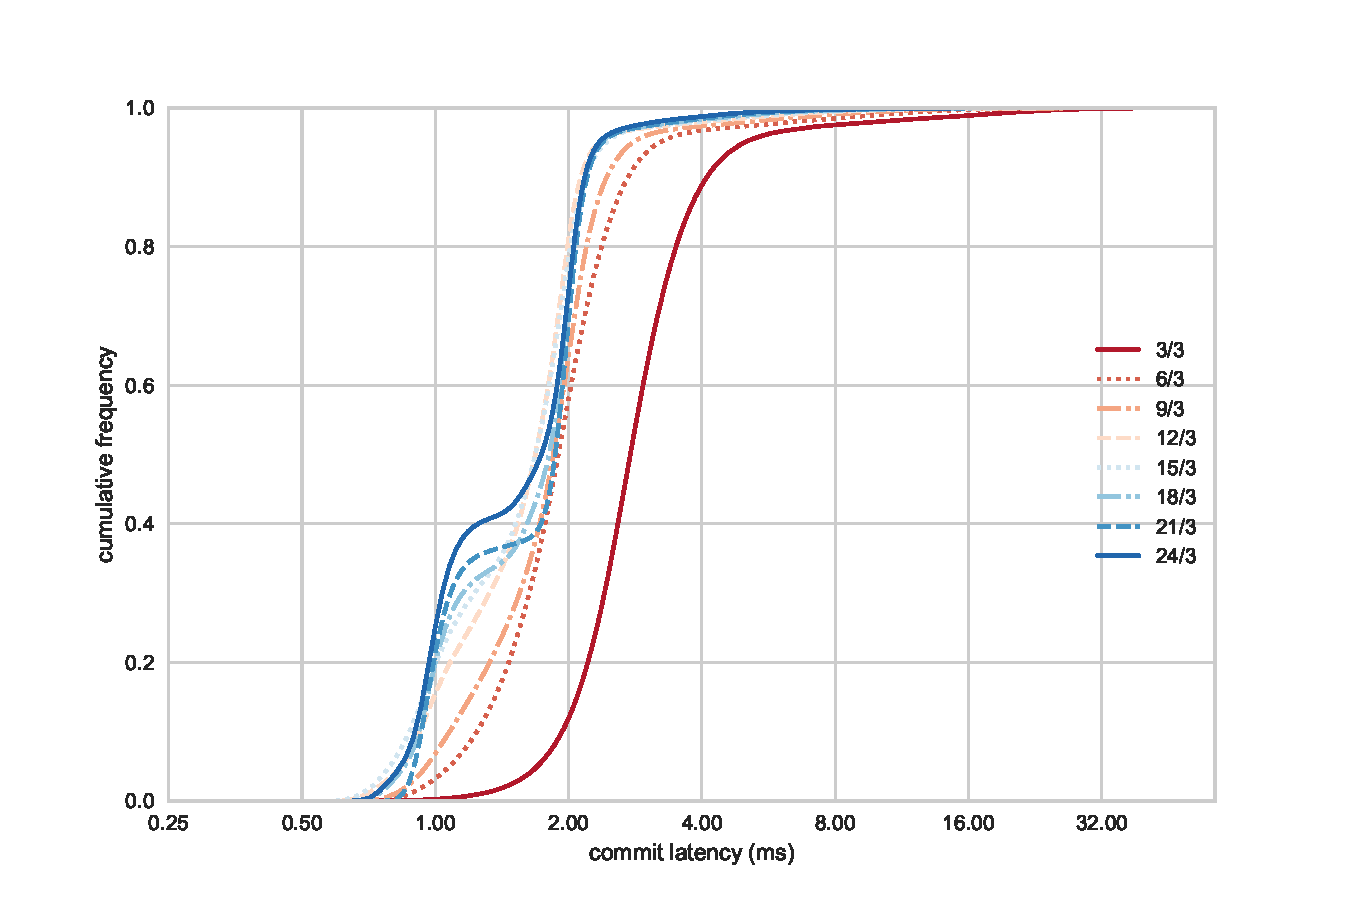
\includegraphics[width=0.48\textwidth]{figures/ec2_latency_cumfreq.pdf}
    \caption{Comulative latency of requests}
    \label{fig:latency}
\end{figure}

The effect of saturation is also demonstrated in Figure~\ref{fig:latency}, which shows 
cumulative latency distributions for different system sizes holding the  workload 
(number of concurrent clients) constant.
The fastest (24/3) shows nearly 80\% of client write requests being serviced in under 
2 msec.
Larger system sizes are faster because the smaller systems suffer from contention (25 
clients can saturate a single subquorum).
Because throughput is directly related to commit latency, throughput variability can be 
mitigated by adding additional subquorums to balance load.

\subsection{Adaptibility}

\begin{figure*}[t]
    \centering
    \minipage{0.5\textwidth}
        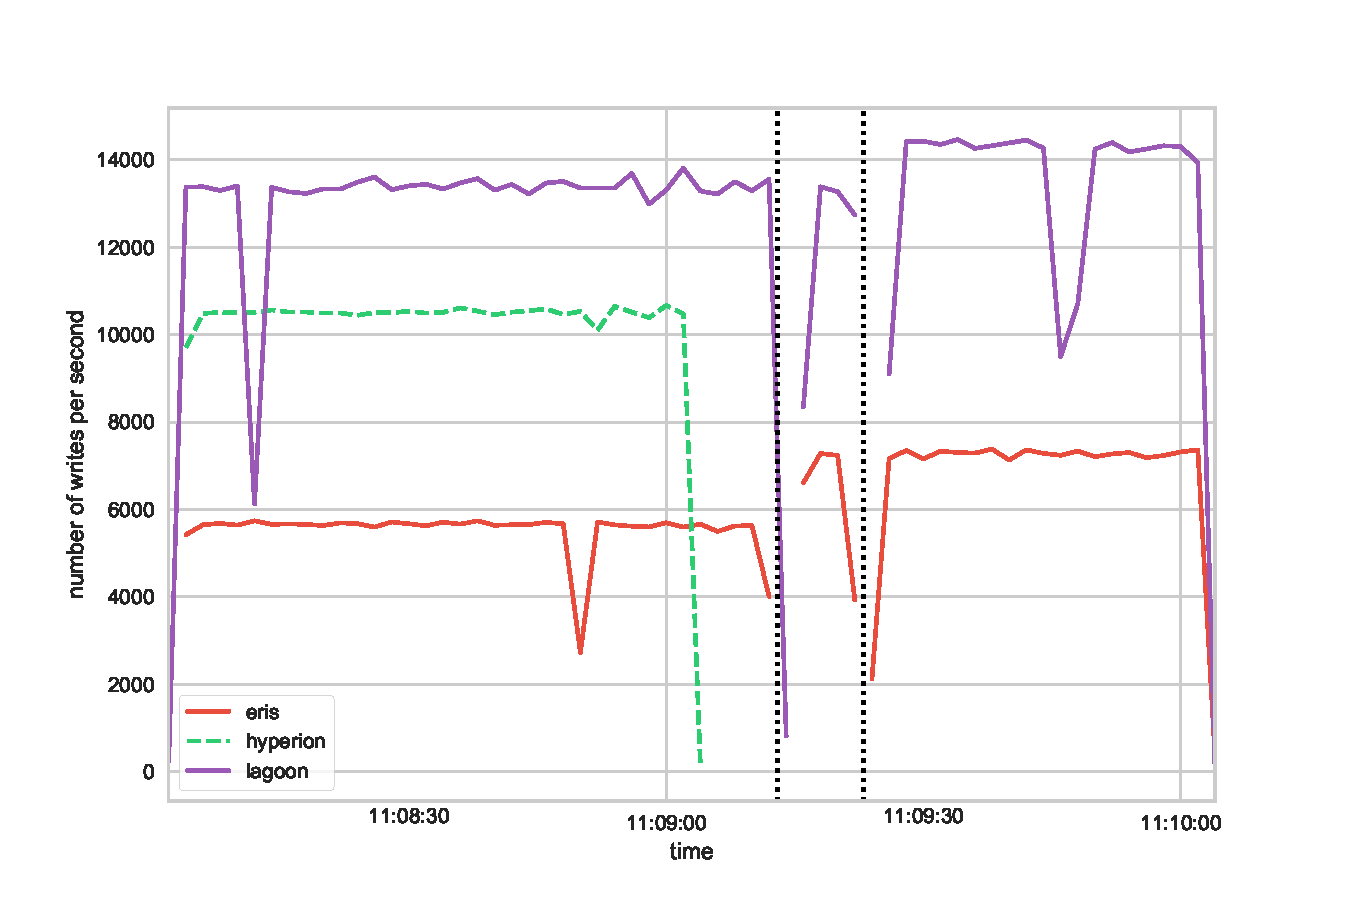
\includegraphics[width=\linewidth]{figures/umd_fault_tolerance.pdf}
        \caption{Reconfiguration to adapt to changing access patterns}
        \label{fig:fault_tolerance}
    \endminipage\hfill
    \minipage{0.5\textwidth}%
        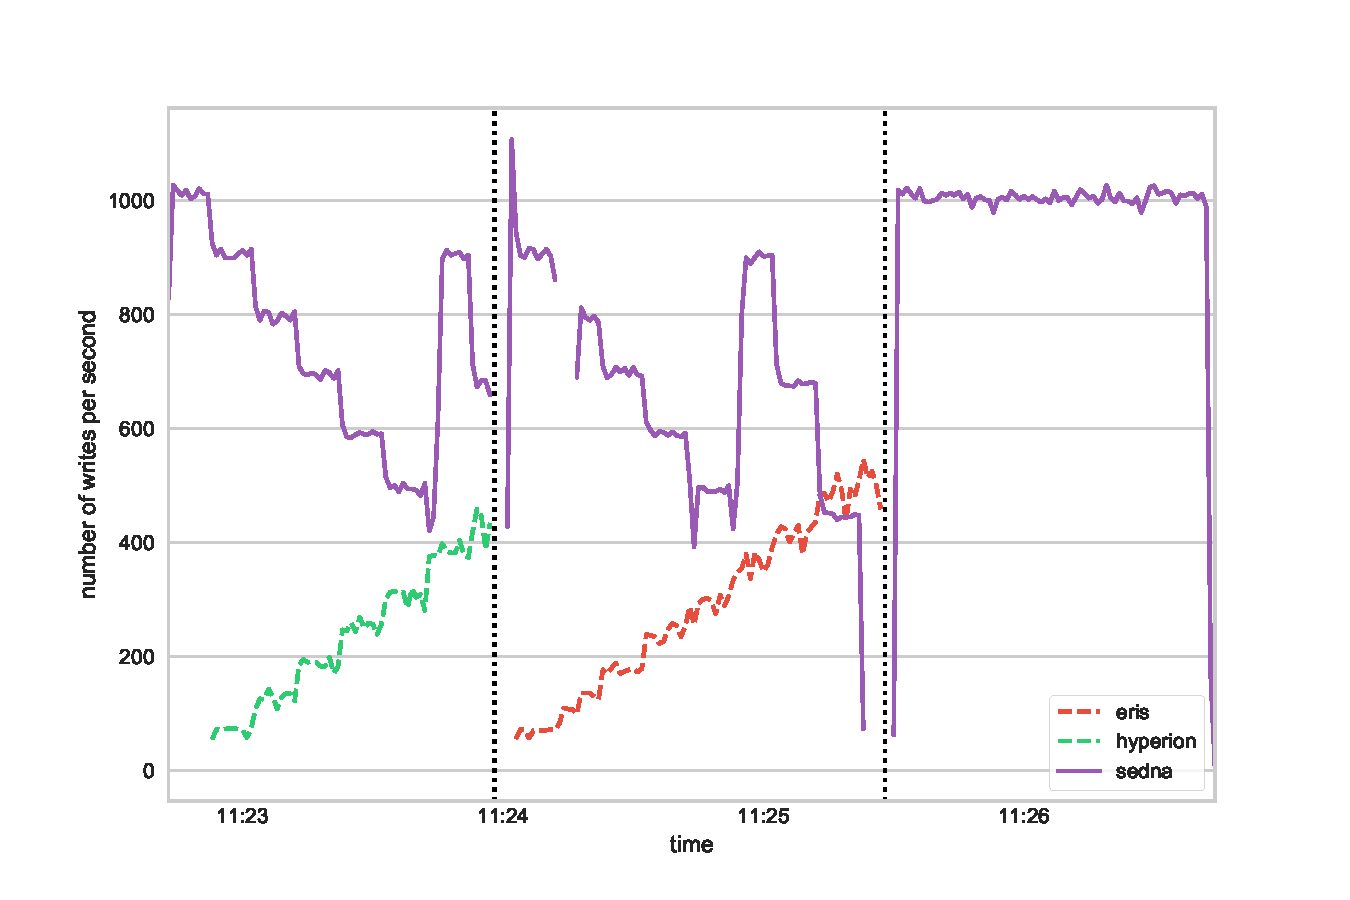
\includegraphics[width=\linewidth]{figures/umd_sawtooth.pdf}
        \caption{Reconfiguration to take over from failing subquorums}
        \label{fig:sawtooth}
    \endminipage
\end{figure*}

Besides pure performance and scaling, HC is also motivated by the need to adapt to 
varying environmental conditions.
In the next set of experiments, we explore two common runtime scenarios that motivate 
adaptation: shifting client workloads and failures.
We show that HC is able to adapt and recover with little loss in performance. These 
scenarios are shown in Figures~\ref{fig:sawtooth} and 
\ref{fig:fault_tolerance} as throughput over time, where vertical dotted 
lines indicate an epoch change.

The first scenario, described by the time series in Figure~\ref{fig:fault_tolerance} 
shows an HC 3-replica configuration moving through two epoch changes.
Each epoch change is triggered by the need to localize tags accessed by
clients to nearby subquorums.
% The experiment was run over machines with widely varying latency.
The scenario shown starts with all clients co-located with the subquorum serving the tag 
they are accessing.
However, clients incrementally change their access patterns first to a tag located on 
one remote subquorum, and then to the tag owned by the other.
In both cases, the root quorum adapts the system by repartitioning the tagspace such 
that the tag defining their current focus is served by the co-located subquorum.

Figure~\ref{fig:fault_tolerance} shows a 3-subquorum configuration where one 
entire subquorum becomes partitioned from the others.
After a timeout, the root uses an epoch change to re-allocate the tag of the partitioned 
subquorum over the two remaining subquorums.
The partitioned subquorum eventually has an heuristic \emph{obligation timeout}, after 
which the  root quorum is not obliged to leave the tag with the current subquorum.
The tag may then be re-assigned to any other subquorum.
Timeouts are structured such that by the time an obligation timeout fires, the root 
quorum has already re-mapped that subquorum's tag to other subquorums.
As a result, the system is able to recover from the partition as fast as possible.
In this figure, the repartition occurs through two epoch changes, the first allocating 
part of the tagspace to the first subquorum, and the second allocating the rest of the 
tag to the other.
Gaps in the graph are periods where the subquorums are electing local leaders.
This may be optimized by having leadership assigned or maintained through root consensus.

\subsection{Planet Scale Consensus}

\begin{figure}
    \centering
    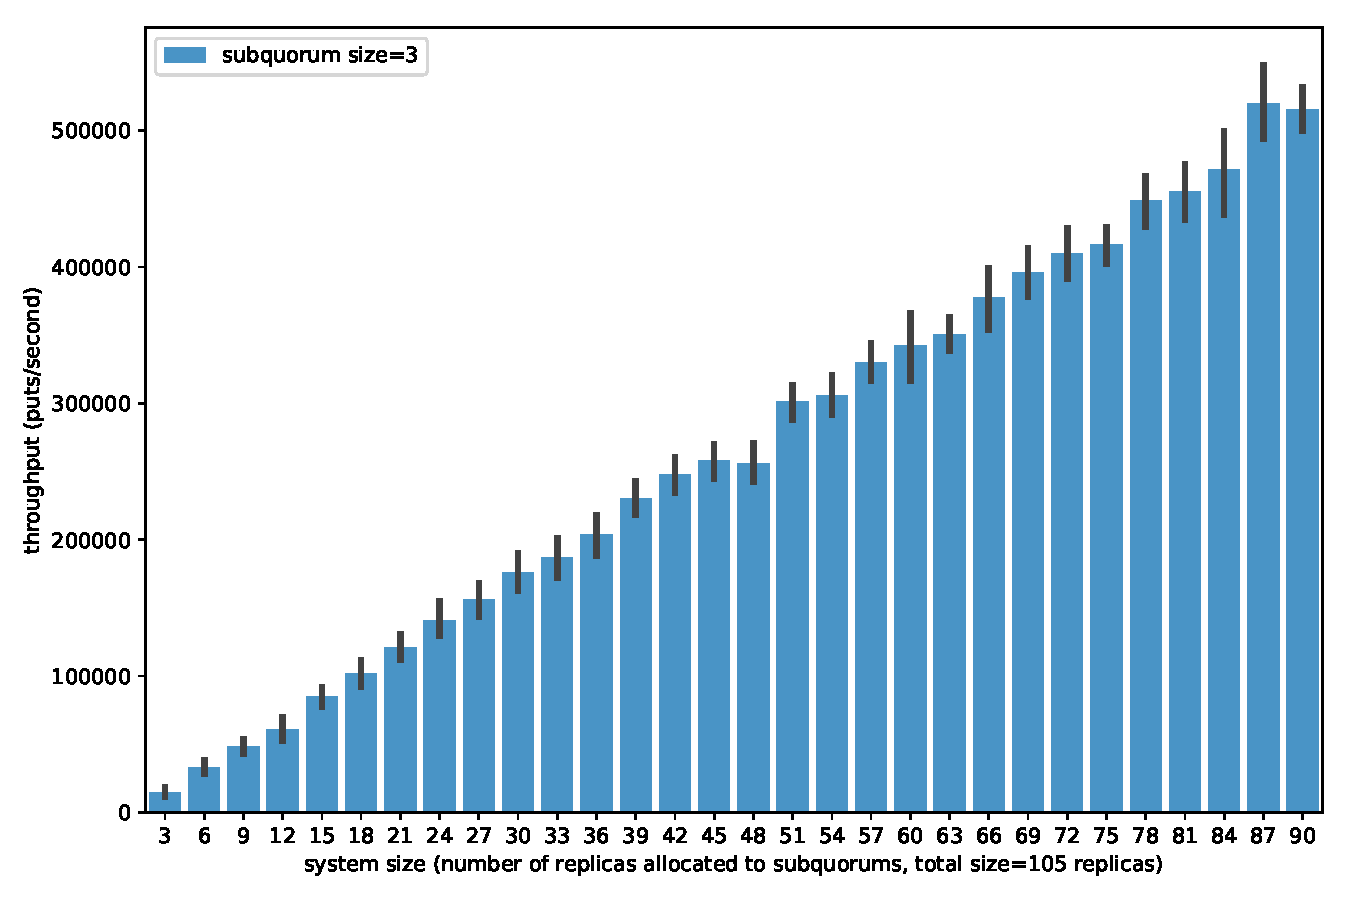
\includegraphics[width=0.48\textwidth]{figures/geoconsensus_throughput}
    \caption{Consensus scales linearly as the number of replicas increases.}
    \label{fig:geoconsensus_throughput}
\end{figure}

In our final implementation we ran our repaired version of HC at a planetary scale.
We created a system with 105 replicas in 15 regions in 5 continents.
The system allocated size 3 subquorums round-robin to each region such that the largest s
ystem was comprised of 6 subquorums per region with 1 hot-spare per region.
Figure~\ref{fig:geoconsensus_throughput} shows the global blast throughput of 
the system, the sum of throughput of client process that fired off 1000 concurrent 
requests, timing the complete response.
To mitigate the effect of global latency, each region ran independent blast clients to 
its local subquorums, forwarding to remote quorums where necessary.
To ensure that the system was fully throttled during the throughput experiment, we timed 
the clients to execute simultaneously using the AWS Time Sync service to ensure that 
clocks were within 100 nanoseconds of each other.
In these results we show that our HC implementation does indeed scale linearly.
Adding more nodes to the system increases the fault tolerance (e.g. by allocating hot s
pares) if enough nodes are added to add another subquorum, the capacity of the system to 
handle client requests is also increased.

\section{Discussion}

Alia takes a different approach to implementing geo-distributed systems, focusing
on a system's ability to be \emph{flexible}.
Flexibility ensures that the system can balance requirements for throughput and
availability while still maintaining the strongest possible consistency semantics.
To achieve this, Alia is based on three primary design requirements that inform the
rest of the framework.

\emph{Requirement 1: Systems should be as fluid as the information they contain.}
Many systems are optimistic, they assume that conflict is rare and that objects are
accessed in standard patterns that change.
In our experience, both people and information flows freely therefore a system must
accommodate organic and shifting usage patterns; for example a set of objects may
primarily be accessed only in daylight, requiring the system to adapt by moving the
coordinating replicas to the locales currently in working hours.
To accommodate this requirement, Alia is designed to regularly and safely transition
through reconfigurations called epoch changes, reallocating replicas into subquorums
to manage specific partitions of the namespace.
Epoch changes are \emph{fuzzy} to ensure that reconfiguration does not need to be
synchronous and hand-offs are optimized through anti-entropy replication of data.

\emph{Requirement 2: No partial failures.}
A system's size should be its advantage -- allowing increased throughput with linear
scaling, and better placement to optimize accesses.
Often, however, a system's size increases its complexity and it's susceptibility
to unique failures such as correlated cascading failure.

Alia is designed with a single process model -- the same process participating in
the root quorum also handles messages for the subquorum(s) the process has been
assigned to.
This model ensures that if a replica fails it cannot participate in some decision
making, such as configuration, but not others, such as accesses.
This requirement also allows us to more easily tackle complex failures; such as
using a nuclear option (discussed in 5.3) to ensure progress even with a worst-case
failure of delegates, or ensuring that leases are either respected or replaced
for whole subquorums that fall out of communication.

\emph{Requirement 3: Consistency semantics must be transparent and interpretable.}
As privacy and security become increasingly important requirements of distributed
systems, consistency is no longer about ensuring that your boss cannot see your
Spring Break pictures on a social network wall.
Instead, consistency is about ensuring that the correct operations are being
executed on the correct replicas and that data can be audited to discover its
exact placement.
Alia ensures that there is an intersection between subquorums where data accesses
are taking place and the root quorum where configuration and namespace partitions
are occurring.
This intersection is optimized by delegated voting to ensure that the root
quorum can make progress and remain fluid.
The intersection also guarantees that a complete, externalizable log of events
for the global system can be exported on demand.

% broadly: fluidity, adaptivity, transparency, bigness
% another item about how size is an advantage to leverage rather than a problem to cope with, an opportunity to scale without adding complications...

% need segue to HC section

% Unused content for Agile Systems subsection
% Wants:
% - Ability to easily modify participants in the system.
% - Detectable failure modes.
% - Responsiveness to changing access patterns
% - Recoverability and ease of maintenance
% - Strong consistency and transactions
% There exists many processes each of which are running in an availability zone in multiple regions.
% Read-write accesses happen to objects according to geographic patterns - single region, multiregion, etc.
% System wants to replicate these accesses to maintain a minimum amount of durability, e.g. protect from a zone failure; but it's not total replication.


\section{Conclusion}

The next generation of distributed systems will be geographically replicated around the
planet in order to provide better performance by preventing bottlenecks and localizing
accesses to international and highly mobile users and to provide durability in the face
of catastrophic failure.
We have presented \hc, an implementation and extension of Vertical Paxos, that is
designed to scale coordination and transparently provide strong consistency in order to
build and deploy systems that span globe.
\Hc is a framework of intersecting tiers of quorums whose primary benefit is flexiblity,
which allows large systems to dynamically adapt to changing conditions, improving both
performance and maintainability.

\Hc handles challenges of geo-distributed consensus through flexible reconfiguration.
Increasing network distance between replicas increases latency and the probability of
network partitions, making strong consistency a challenge.
To handle this, we separate the concerns of placement and access decisions to the \roo
and \subs, allowing as much of the system to operate as independently as possible.
Centralized administration is impossible in a global context, so the \roo is able to
adapt the system automatically by observing conditions and applying policy-driven
changes to the system in real time with fuzzy transitions.
To ensure correct reasoning of global consistency semantics and reduce the complexity of
independent-subsystems with different failure modes, \hc ensures that there is an
intersection of the \roo and subs.
This interesection requires all nodes to participate in the root quorum, so to scale
this quorum, we introduce delegated volding to improve globably availability.
Finally, because objects have different requirements for availability or durability,
data placement rules and subquorum behavior can be adjusted for different geographic
access patterns.

% Future work:
% - investigate the affect of more tiers of consensus
% - transactions
% - automatic adaptibility using learning rather than policies and heuristics

\bibliographystyle{plain}
\bibliography{papers}

\end{document}